\subsection{Technology}%TODO: Make all sub(sub)sections of this document conform to one standard (ie. start the same, same structure etc.)

This subsection covers the technology we utilized during our project. It covers the various operating systems our group members have been working on, editors and IDEs for documents and code, as well as frameworks and platforms used in development. Additionally it covers tools for version control and file sharing between the group members, as well as communication platforms.

\subsubsection{Windows 7, 8}
Microsoft Windows 7 and - 8 are operating systems by the Microsoft Corporation. They logically provide good support for .NET developments, seeing as .NET targets the Windows platform and is made by Microsoft. Visual Studio is made for Windows, and was our main IDE, so all group members had access to PCs with Windows installed.

\subsubsection{Ubuntu Linux}
This OS is perhaps the most widely used distribution of Linux, developed by Canonical Ltd. It provides good support for many development tools, except of course Windows development. However we did find support for using it for some Windows development.
This operating system was used by one group member on a laptop, when working on-site at NTNU. For coding, Mono with MonoDevelop was used, while other tasks were mostly unaffected. The operating system provides good support for other parts of the process, such as Git and \LaTeX.

\subsubsection{OS X}
OS X\footnote{http://en.wikipedia.org/wiki/OS\_X}
 is the main operating system for the Macs developed by Apple. It is based on the Mach kernel and as Ubuntu Linux it provides good support for many development tools, except Windows development. One of our group members is running OS X. He used OS X for writing documentation and rebooted to Windows when writing code. 

\subsubsection{Visual Studio 2012}
Visual Studio is Microsofts IDE for development for their platforms. This is the main IDE we developed the framework on, seeing as it has very good integration with C\# and .NET platforms, which we were required to use. We decided to use the ultimate version because this version provides everything we might need.

\subsubsection{.NET and Mono}
We were required to use ASP .NET MVC for our framework. ASP .NET MVC is a framework for web applications which enables the use of the Model View Controller (MVC) pattern. It is part of Microsofts .NET Framework suite, which is the preferred way of interactiong with Windows systems and OSes.

Mono is the open source-, cross-platform version of the .NET suite, which we used when not developing on Windows machines. It is available both for Windows, OS X, most Linux Distributions, Android, and various other operating systems.

\subsubsection{MonoDevelop}
This is an open source IDE for development with Mono, available for OS X and most Linux distributions. This was the IDE used when not developing on Windows machines.

\subsubsection{Google Chrome with Developer Tools}
%%TODO Write about Chrome and its developer tools, which we used for testing of Web API methods.

\subsubsection{Doxygen}
Doxygen is a documentation generator that generates software reference documentation directly from source file comments and tags. It supports multiple programming languages, and outputs documentation in several formats, including, but not limited to: HTML, {LaTeX},and man pages.

We used Doxygen in our project to generate the API documentation requested by the customer. It was chosen due to easy setup and configuration, support for C\#s XML-comments and tags, as well as multi-platform support (Windows, Linux and Mac OS X).

\subsubsection{\LaTeX}
We quickly chose \LaTeX \ for our typesetting, due to it being the de-facto standard for academic typesetting, with good support for both code snippets, tables, references and bibliography.

Most of our group also had at least some experience using it, and some were quite experienced, which made the choice easier.

\subsubsection{Git}
For our version control and source repository, we chose Git. This because we had most experience with it, and found it easy to set up via GitHub (where we all had accounts already). It also has the advantage of being distributed, so we could avoid a single point of failure, and having a staging area where one can selectively commit files according to whether they're ready or not, instead of risking accidental changes which might break something.

Both the source code and the entirety of the report source files were stored on GitHub, since both would be catastrophical to lose, and were quite important to have under version control in case we needed to track problematic changes.

To communicate with GitHub, we used various tools. Some of us used the built in terminal with git installed, and some of us used GitBash. Git for windows was also used on rare occasion.

\subsubsection{Trello}\label{Trello}
To support our agile process and sprints, we used Trello for planning and control of work flow. It is an online Scrum Board tool, where we can create work packages and issues, while tracking who does what, and tracking backlog, finished modules, and work in progress.

\begin{figure}[H]
\centering
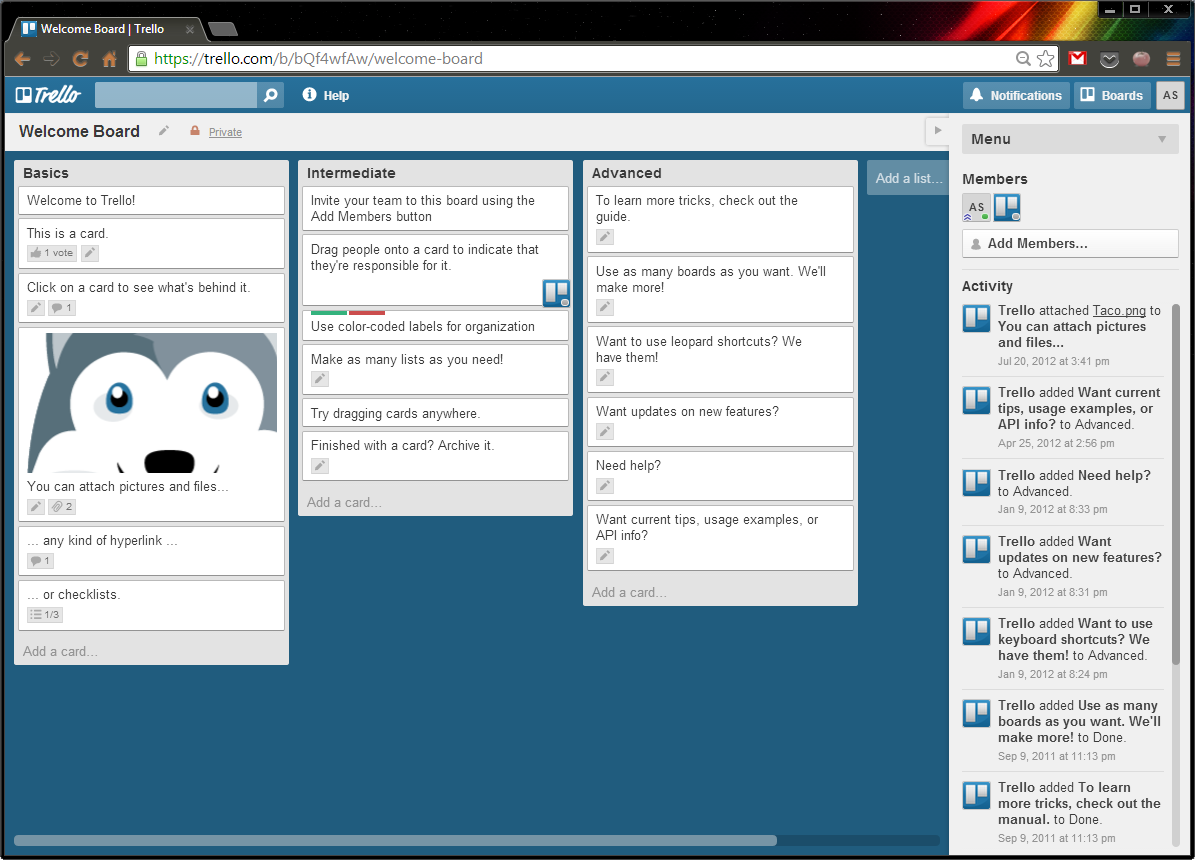
\includegraphics[width=0.8\textwidth]{images/Trello.png}
\caption{Example Trello Board}
\label{fig:Trello}
\end{figure}

The above figure shows an example Trello board. You create cards (tasks) and lists to contain and separate those cards into categories, such as \emph{Backlog}, \emph{ToDo}, \emph{In Progress}, \emph{Testing} and \emph{Completed}. The tasks can be assigned to the members of the board, and there are handy functions available such as adding check lists to cards to keep track of sub-tasks.

\subsubsection{Web API}

ASP.NET Web API is a framework for building web APIs on top of the .NET Framework, it lets you create calls from the browser to the methods in the code, this can be done via parameters or via JSON. The web API framework returns a JSON-format of the given item, table or whatever was requested.

\subsubsection{Dropbox}
\href{http://www.dropbox.com}{Dropbox} is a syncing service that let you choose a local folder on your machine that will be synced to the cloud. Dropbox lets you share folders and files inside a shared Dropbox folder.

We used Dropbox for sharing and synchronizing internal documents that usually were only useful for a limited time, but might be referenced later.

\subsubsection{Google Drive}
\href{https://drive.google.com/}{Google Drive} is Google's productivity suite/office pack. The difference between Drive and other office solutions (like Microsoft Office, OpenOffice/LibreOffice) is that Drive exists in the cloud and lets the user simultaneously work on a document.

Google Drive was used for simultaneous collaboration on documents, where the content was up for discussion, or it was advantageous to see what the others where writing, as well as for dynamic internal documents like work logs.

\subsubsection{Microsoft SQL server}
The customer uses Microsoft SQL server as their database, and we received a backup dump of their database. MSSQL is a relational database management system developed by Microsoft. The first version of MSSQL was released back in 1989 - a 16 bit version for OS/2 \footnote{http://en.wikipedia.org/wiki/OS/2}. The latest version of MSSQL is MSSQL version 11 (called MSSQL Server 2012 - codename Delali). There will be a new version coming out in 2014 - MSSQL Server 2014 (version 12).

\subsubsection{Entity Framework}
The customer's preference was that we utilized Microsoft's entity framework to connect to the database. The entity framework is an object-relational mapper that enables .NET developers to access the database without writing the typical data-access code that developers typically need to write. EF lets the developer work with domain specific object and properties without worrying about the underlying database table.

\subsection{Extra Tools}
\subsubsection{\LaTeX \ Editors}%TODO: Possibly reduce info detail in this section
We have used several editors for our \LaTeX \ documents. Some members have used TeXstudio, others have used TeXworks, while others again have used Gummi.

TeXworks is a simple, lightweight working environment for \LaTeX \ documents, and is modeled on TeXShop. It provides several compilers, and a raw text editor, as well as a pdf viewer, but little else.

TeXstudio, a fork of Texmaker, is better described as an integrated development environment (IDE). Relative to TeXworks, it better supports simultaneous work on several \LaTeX \ documents. It also supplies multiple compilers, a pdf viewer and a text editor, but it includes some nice-to-have features that are not available in TeXworks. Some examples of these features are:
\begin{itemize}
\item Easy navigation between included files
\item Compilation of main document directly from included files
\item View included images through hover
\item Keyboard shortcuts for often used functions
\end{itemize}

Gummi is a free, open-source, lightweight working environment for \LaTeX \ which is available in the repositories of most widely used Linux distributions, and for Windows as well. It provides live preview of the document without manual compilation, support for multiple compilers, bibliography management, and SyncTeX support. It also provides easy insertion of tables and images.

\subsubsection{\LaTeX \ Compilers}
We have also used several \LaTeX \ compilers, most notably pdfLaTeX and BibTeX. We have used BibTeX specifically to handle citations and references, and pdfLaTeX for general compilation of our documents.

\subsubsection{Git Tools}
We have used various tools for Git, such as Git Bash and GitHub For Windows, as well as Git for Linux. GitHub For Windows is a graphical user interface for Git, and provided good visualization of branching, while Git Bash and Git for Linux were used for straight-forward commit, pull and push.

\subsubsection{LibreOffice Calc}
%TODO HD

\subsubsection{Raw Text Editors}
A variety of raw text editors were used, mainly for meeting notes and similar small and temporary documents. Sublime Text was used by most of the group, allowing us to read and edit text files with no file ending. Some also chose to use gedit.

\subsubsection{Communication}
Various software was used for communication when the group members were at separate locations. Foremost of these were Facebook Messenger and e-mail. We also used IRC, to which some connected through means such as PuTTY, to connect through ssh to a server running irssi in screen, while others ran mIRC locally or connected through ssh in another terminal (such as the native terminal of their OS).
